\documentclass[9pt]{beamer}

\usepackage{appendixnumberbeamer}
\usepackage{booktabs}
\usepackage[scale=2]{ccicons}
\usepackage{pgfplots}
\usepackage{tikz}
\usepackage{graphics}

\usepgfplotslibrary{dateplot}
\pdfstringdefDisableCommands{\def\translate#1{#1}}
\geometry{paperwidth=140mm, paperheight=105mm}
\usetheme{metropolis}
\bibliographystyle{abbrv}
\setbeamertemplate{frame footer}{Lab - Mechatronics}

\usetikzlibrary{shapes, arrows}
\tikzstyle{startstop} = [rectangle, rounded corners, minimum width=2cm, minimum height=1cm, text centered, draw=black, fill=red!30]
\tikzstyle{io} = [trapezium, trapezium stretches=true, trapezium left angle=70, trapezium right angle=110, minimum width=2cm, minimum height=1cm, text centered, draw=black, fill=blue!30]
\tikzstyle{process} = [rectangle, minimum width=2cm, minimum height=1cm, text centered, text width=2cm, draw=black, fill=orange!30]
\tikzstyle{decision} = [diamond, minimum width=2cm, minimum height=1cm, text centered, draw=black, fill=green!30]
\tikzstyle{arrow} = [thick,->,>=stealth]

\title{Modelling and control of a Magnetic Levitation System}
% \subtitle{Tie-rods case study}
\date{\today}
\author{Tommaso Bocchietti 10740309 \\ Sara Orazzo 10??????}
\institute{Politecnico di Milano}
\titlegraphic{\hfill
\includegraphics[height=1.5cm]{pdf/Polimi_logo_header.pdf}}

\begin{document}

\maketitle

\begin{frame}{Agenda}

    \begin{columns}[c, onlytextwidth]

        \begin{column}{0.5\textwidth}

            \setbeamertemplate{section in toc}[sections numbered]
            \tableofcontents

        \end{column}

        \begin{column}{0.5\textwidth}

            \begin{figure}[H]
                \centering
                % https://www.researchgate.net/publication/354123381_Comparison_of_Nonlinear_and_Linear_Controllers_for_Magnetic_Levitation_System
                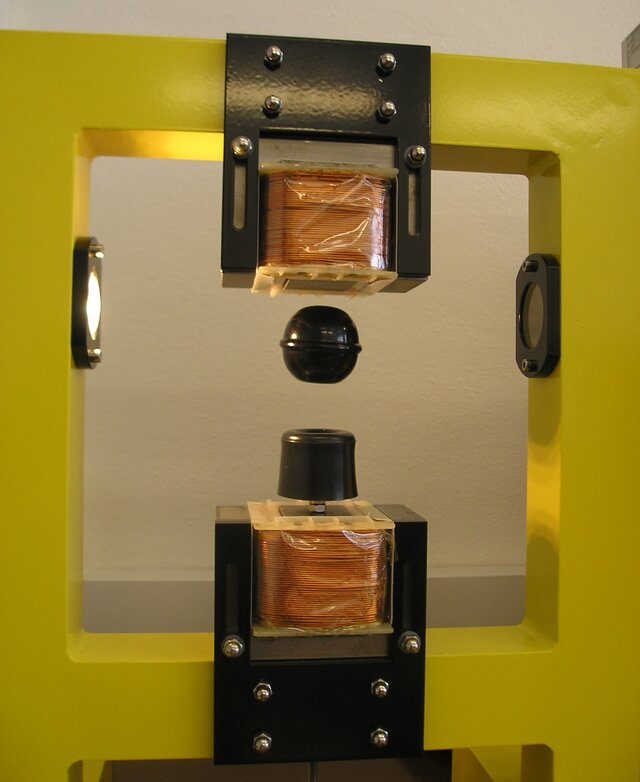
\includegraphics[width=0.8\textwidth]{img/ML2SEM magnetic levitation equipment.jpg}
                \caption{Magnetic Levitation System}
            \end{figure}

        \end{column}

    \end{columns}

\end{frame}


% \input{src/01 - problem_statement}
% \input{src/02 - proposed_solutions}
% \input{src/03 - results}
% \input{src/04 - conclusions}
% \input{src/05 - extra_slides}

\appendix

\begin{frame}[allowframebreaks]{References}
    \nocite{*}
    \bibliography{references}
\end{frame}

\begin{frame}[standout]
    Questions?
\end{frame}

\begin{frame}[standout]
    Thank you!
\end{frame}

\end{document}